% arara: pdflatex: { shell: true, draft: true }
% arara: makeglossaries
% arara: biber
% arara: pdflatex: { shell: true, synctex: true }
% arara: pdflatex: { shell: true, synctex: true }

\documentclass{f4_beamer_metropolis}

\title{Transport Layer Security 1.3}
\subtitle{SITS WS18/19}
\author{Dennis Grabowski, B.Sc}
\date{28.11.2018}

\bibliography{literature.bib}

\begin{document}

% Cannot be moved into the class
\begin{frame}{Inhaltsverzeichnis}
    \tableofcontents[hideallsubsections]
  \end{frame}

\section{Einfuehrung}

\begin{frame}{Was ist Transport Layer Security (TLS)?}
  \begin{itemize}
    \item Hybrides Verschlüsselungsprotokoll zur sicheren Datenübertragung im Internet
    \item Liegt zwischen Transport Layer und Application Layer im TCP/IP-Stack
    \item \textbf{Nicht} nur fuer HTTP(S): POP3\textbf{S}, SMTP\textbf{S}, IMAP\textbf{S}, XMPP\textbf{S}, IRC\textbf{S}, FTP\textbf{S}, OpenVPN...
    \item Verbesserung des alten \enquote{Secure Sockets Layer (SSL)}-Protokolls
    \item TLS 1.0 im Januar 1999 als Upgrade zu SSL 3.0 entwickelt wurden
    \item Aufgeteilt in \enquote{Teil}-Protokolle:
  \end{itemize}
  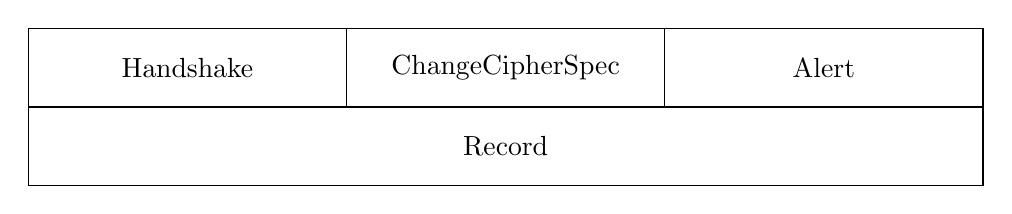
\begin{tikzpicture}
    \draw (0,0) rectangle (\textwidth, 1) node[pos=.5] {Record};
    \draw (0, 1) rectangle (\textwidth / 3,2) node[pos=.5] {Handshake};
    \draw (\textwidth / 3, 1) rectangle (\textwidth / 3 + \textwidth / 3, 2) node[pos=.5] {ChangeCipherSpec};
    \draw (\textwidth / 3 + \textwidth / 3, 1) rectangle (\textwidth / 3 + \textwidth / 3 + \textwidth / 3, 2) node[pos=.5] {Alert};
  \end{tikzpicture}

  \note{
    Von der Basis auf TCP kommt der Name Transport Layer Security.
    Record Protokoll: Arbeitet mit den eigentlichen Daten vom Application Layer, verschluesselt diese, fragmentiert sie falls noetig und sendet sie zum Transport Layer, zusaetzlich ist Kompression moeglich.
    Alert Protokoll: Gibt Status an Gegenueber weiter: Fehler, Connectionabbrueche, etc.
    Handshake Protokoll: Kuemmert sich um die Authentifizierung sowie Schluesselaustausch und stellt eine Verbindung zwischen Client und Server her.
    ChangeCipherSpec Protokoll: Kann genutzt werden, um die Verschluesslung zu wechseln.
  }
\end{frame}

\subsection{Motivation}

\begin{frame}{TLS 1.2}
Release: \textbf{vor 10 Jahren} \\
Letzte Aenderungen dazu durch:
\begin{itemize}
    \item RFC6176, veroeffentlicht in \textbf{\citeyear{RFC6176}}: \newline
    \textit{\citetitle{RFC6176}}
    \item RFC7627, veroeffentlicht in \textbf{\citeyear{RFC7627}}: \newline
    \textit{\citetitle{RFC7627}}
    \item RFC7685, veroeffentlicht in \textbf{\citeyear{RFC7685}}: \newline
    \textit{\citetitle{RFC7685}}
\end{itemize}
\end{frame}

\begin{frame}{Welche neuen, relevanten Technologien wurden entwickelt?}
  \begin{itemize}
    \item HTTP Public Key Pinning (HPKP) \autocite{RFC7469}
    \item Certificate Transparency (CT) \autocite{RFC6962}
    \item TLS False Start \autocite{RFC7918}
    \item Hash Key Derivation Function (HKDF) \autocite{RFC5869}
    \item Curve25519 sowie 448 \autocite{RFC7748}
    \item Edwards-curve Digital Signature Algorithm (EdDSA) \autocite{RFC8032}
    \item SHA3
  \end{itemize}

  \note{
    Disclaimer: Curve22519 is not a new technology.
    It was released in 2005.
    But after discovery that NSA implemented a backdoor into Dual\_EC\_DRBG, interest increased.
    Since 2017 NIST added them to Special Publication 800-186, allowing the use by US Federal Government.
  }
  \end{frame}

\begin{frame}{Welche Angriffe wurden seit TLS1.2 Release gefunden?}
  \begin{itemize}
    \item \textbf{Implementationsfehler}: Heartbleed, BERserk
    \item \textbf{\enquote{Downgrading}-Angriffe:} FREAK \& Logjam
    \item \textbf{\enquote{Cross-protocol}-Angriffe:} DROWN, Unholy PAC
    \item \textbf{\enquote{Chosen-plaintext}-Angriffe:} BEAST
    \item \textbf{Kompressions-basierte Angriffe:} CRIME, TIME, \& BREACH
    \item \textbf{\enquote{Padding oracle}-Angriffe:} POODLE, Serge Vaudenay's Angriff, Bleichenbacher's Oracle Angriff (ROBOT)
    \item \textbf{Timing-Angriffe:} Lucky Thirteen
    \item \textbf{Side-Channel-Angriffe:} HEIST
    \item \textbf{Angriffe auf spezifische Chiffre:} Sweet32, ROCA
    \item \textbf{Angriffe auf spezifische Hashing-Funktionen:} SLOTH, RC4
    \item \textbf{\enquote{Renegotiation}-Angriffe:} 3SHAKE
    \item \textbf{\enquote{Truncation}-Angriffe}
    \item \textbf{Resumption-basierte Angriffe}
  \end{itemize}

  \note{
    RC4 Cipher attacks esp. bad in timing as it was recommended as mitigation against BEAST \\
    PKCS\#1 v1.5 sowie CBC ciphers ist oftmals Ursprung der Padding Oracle Angriffe.
    SHA1-Angriff SHAttered
  }
\end{frame}

\section{TLS 1.3}

\begin{frame}{TLS1.3}
  \begin{itemize}
    \item Release in August \citeyear{RFC8446}
    \item Spezifikation in RFC8446: \textit{\citetitle{RFC8446}}
    \item IETF began August 2013 mit ersten Arbeiten an TLS 1.3
    \item Erster Draft in April 2014 veroeffentlicht wurden
    \item Unter anderem daran beteiligt:
    \begin{itemize}
      \item Google, Cloudflare, Akamai, Vodafone, Mozilla, Apple, Microsoft, Amazon, Facebook, Red Hat, IBM, ANSSI, Sun Microsystems, Nokia, Symantec, OpenSSL, Cisco...
    \end{itemize}
    \item Aufgrund signifikanter Aenderungen beinahe TLS 2.0 oder gar 4.0 genannt\footnote{\url{https://www.ietf.org/mail-archive/web/tls/current/msg20938.html}}
  \end{itemize}

  \note{
    ANSSI = franzoesischer Geheimdienst
  }
\end{frame}

\newcolumntype{Y}{>{\centering\arraybackslash}X}
\newcolumntype{S}{>{\centering\small}X}

\subsection{Browser- und Bibliotheksunterstuetzung}

\begin{frame}{Welche Browser unterstuetzen TLS 1.3?}
  \begin{tabularx}{\textwidth}{
      |>{\hsize=0.2\hsize} Y |
      >{\hsize=0.5\hsize} S |
      >{\hsize=0.2\hsize} Y |
      >{\hsize=0.1\hsize} Y |
    }
    \hline
    \textbf{Browser} & \textbf{Platforms} & \textbf{Versions} & \textbf{TLS 1.3}\\ \hline
    \multirow{2}{*}{Google Chrome}
        & \multirow{2}{*}{\parbox{6cm}{Windows (7+), Linux, Android (4.1+), Chrome OS, macOS (10.10+), iOS (9.0+)}}
          & 54 - 69 & \cellcolor{yellow!50}Disabled \\ \cline{3-4}
    & & 70 & \cellcolor{green!50}Yes \\ \hline
    \multirow{2}{*}[-0.75em]{Mozilla Firefox}
    & \multirow{2}{*}[-0.75em]{\parbox{6cm}{Windows (7+), Linux, Android (4.1+), macOS (10.9+), iOS (9.0+)}}
      & 49 - 62, ESR 52.0 - 60.3 & \cellcolor{yellow!50}Disabled \\ \cline{3-4}
    & & 63 & \cellcolor{green!50}Yes \\ \hline
    Internet Explorer & Windows (7+), Windows Server (2008 R2+) & IE 11 & \cellcolor{red!50}No \\ \hline
    \multirow{2}{*}{Microsoft Edge}
        & Windows 10 Mobile, Xbox & Edge 15 & \cellcolor{red!50}No \\ \cline{2-4}
    & Windows 10, Windows Server (2016+) & Edge 18 & \cellcolor{red!50}No \\ \hline
    Apple Safari & iOS 12, macOS 10.14 & 12 & \cellcolor{yellow!50}Disabled \\ \hline
    Opera Browser & Windows (7+), Linux, Android (4.0+), macOS (10.9+) & 56 & \cellcolor{yellow!50}Disabled \\ \hline
    Tor Browser & Windows (7+), Linux, macOS (10.9+) & IE 11 & \cellcolor{green!50}Yes \\ \hline
    \end{tabularx}

    \note{
      Chrome uses BoringSSL (Google's fork of OpenSSL) \\
      Firefox uses Mozilla's Network Security Services (NSS) \\
      Edge uses Microsoft's EdgeHTML on Windows, Apple/KDE's Webkit on iOS, and Chromium's Blink on Android \\
      Opera uses Apple/KDE's Webkit and Chromium's Blink \\
      Apple Safari apparently allows the use of TLS 1.3, but it is disabled and must be activated with \texttt{defaults write /Library/Preferences/com.apple.networkd tcp_connect_enable_tls13 1}\\
      Tor uses Firefox ESR 60.2 under the hood, which currently only implements the draft-22 version, but they are thinking about backporting NSS changes
    }
\end{frame}

\begin{frame}{Welche Bibliotheken unterstuetzen TLS 1.3?}
  \begin{tabularx}{\textwidth}{
    |>{\hsize=0.4\hsize} Y |
    >{\hsize=0.2\hsize} Y |
    >{\hsize=0.3\hsize} Y |
    >{\hsize=0.1\hsize} Y |
  }
  \hline
  \textbf{Library} & \textbf{Language} & \textbf{Versions} & \textbf{TLS 1.3}\\ \hline
  BoringSSL & C++ & \texttt{master} & \cellcolor{green!50}Yes \\ \hline
  fizz & C++ & v2018.11.12.00 & \cellcolor{green!50}Yes \\ \hline
  GnuTLS & C & 3.6.3 & \cellcolor{green!50}Yes \\ \hline
  Java Secure Socket Extension & Java & JDK11 & \cellcolor{green!50}Yes \\ \hline
  miTLS & F* & - & \cellcolor{green!50}Yes \\ \hline
  NSS & C / Assembler & 3.39 & \cellcolor{green!50}Yes \\ \hline
  OpenSSL & C & 1.1.1 & \cellcolor{green!50}Yes \\ \hline
  rustls & Rust & 0.14.0 & \cellcolor{green!50}Yes \\ \hline
  SChannel (Windows API) & C++ & Windows 10 v1607 & \cellcolor{red!50}No \\ \hline
  Secure Transport & C / Swift & macOS 10.13, iOS 11 & \cellcolor{yellow!50}Yes \\ \hline
  wolfSSL & C & 3.15 & \cellcolor{green!50}Yes \\ \hline
  \end{tabularx}

  \note{
    cryptlib is a library from Peter Gutmann, a Professor in Auckland \\
    JSSE (Java) will need JDK11, but other library like Bouncy Castle is good too. \\
  }
\end{frame}

\subsection{Allgemeine Aenderungen}

\begin{frame}{Allgemeine Aenderungen}
  \begin{itemize}
    \item ChangeCipherSpec wurde entfernt, somit bleibt ueber: \\
    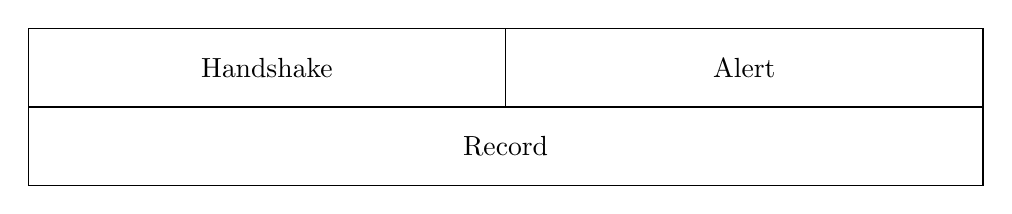
\begin{tikzpicture}
      \draw (0,0) rectangle (\textwidth, 1) node[pos=.5] {Record};
      \draw (0, 1) rectangle (\textwidth / 2,2) node[pos=.5] {Handshake};
      \draw (\textwidth / 2 , 1) rectangle (\textwidth / 2 + \textwidth / 2, 2) node[pos=.5] {Alert};
    \end{tikzpicture}
    \item Renegotiation zu SSL untersagt
    \item Nutzer-definierte Diffie-Hellmann Gruppen nicht mehr unterstuetzt
    \item Nur noch Schluesselaustauschprotokolle, die Perfect Forward Secrecy garantieren:
    \begin{itemize}
      \item DHE-RSA,
      \item ECDHE-RSA,
      \item ECDHE-ECDSA
    \end{itemize}
  \end{itemize}

  \note{
    Entfernen der Custom DHE Groups macht es erst moeglich, dass ein ganzer Round Time Trip vom Handshake entfernt werden kann, da der Client einfach welche zu Beginn des Verbindungsaufbaus auswaehlt und daher nicht erst mit dem Server aushandeln muss, welche benutzt werden muessen
    Erlaubt sind also nur noch die Schluesselaustauschprotokolle, die auf ephemeral Diffie-Hellmann (ueber finite Felder oder elliptic-curve) oder auf einem pre-shared Key aufbauen.
    Das bedeutet, dass statisches RSA oder DSA gar nicht mehr erlaubt ist.
  }
\end{frame}

\subsection{Aenderungen am Handshake-Protokoll}

\begin{frame}{TLS v1.2 Handshake}
  \begin{figure}[!h]
    \centering
    \includegraphics[scale=0.375,keepaspectratio]{./images/tls12-handshake-ecdhe.png}
    %\caption{TLS 1.2 Handshake mit ECDHE}
    \label{fig:tls12-handshake-ecdhe}
    \autocite{taubert}
  \end{figure}

  \note{
    ECDHE daher, weil static RSA ab TLS 1.3 nicht mehr unterstuetzt ist.
    Bei static RSA wuerde ServerKeyExchange nicht durchgefuehrt werden.
    Base Key zum Verschluesseln ab EncryptedExtensions hier ist das \texttt{server_handshake_traffic_secret}
  }
\end{frame}

\begin{frame}[standout]
  TLS v1.2 Handshake - Wiresharkdemo
\end{frame}

\begin{frame}{TLS v1.3 Handshake}
  \begin{figure}[!h]
    \centering
    \vspace*{-0.25cm}
    \includegraphics[width=\linewidth]{./images/tls13-handshake-ecdhe.png}
    %\caption{TLS 1.3 Handshake mit ECDHE}
    \label{fig:tls13-handshake-ecdhe}
    \footnote{\autocite{taubert}}
  \end{figure}

  \note{
    Moeglich, da RSA und Custom DH Groups entfernt wurden.
    Durch festgesetzte finite Gruppen fuer den Diffie-Hellmann Austausch ist es einfach zu entscheiden, welche Parameter wohl vom Server unterstuetzt werden (entweder ECDHE mit x25519, P-256).
    Dadurch kann Client KeyShares direkt mitschicken, es verfaellt das Beduerfnis darueber zu verhandeln und wir sparen uns einen RoundTrip
  }
\end{frame}

\begin{frame}[standout]
  TLS v1.3 Handshake - Wiresharkdemo
\end{frame}

\begin{frame}{0-RTT Handshake}
  \begin{figure}[!h]
    \centering
    \vspace*{-0.25cm}
    \includegraphics[width=\linewidth]{./images/tls13-handshake-zero-rtt.png}
    %\caption{TLS 1.3 Handshake mit ECDHE}
    \label{fig:tls13-handshake-zero-rtt}
    \autocite{taubert}
  \end{figure}
  \note{
    0-RTT sind anfaellig gegenueber Replayattacken
    Muessen daher idempotent sein, wird geraten nur bei GET zu erlauben
    Anwesenden fragen, ob sie eventuell Problem mit dem 0-RTT Handshake sehen
  }
\end{frame}

% \subsection{Session Resumption}

% \begin{frame}{Session Resumption basierend auf einem \enquote{pre-shared key}-Modus}
%   \begin{figure}[!h]
%     \centering
%     \includegraphics[width=\linewidth]{./images/tls13-handshake-resumption.png}
%     %\caption{TLS 1.3 Handshake mit ECDHE}
%     \label{fig:tls13-handshake-resumption}
%     \autocite{taubert}
%   \end{figure}
% \end{frame}

\begin{frame}{Was ist \enquote{downgrading}?}

\end{frame}

\begin{frame}{LogJam Angriff: Ablauf}
  \begin{figure}[!h]
    \centering
    \vspace*{-0.35cm}
    \includegraphics[scale=0.8]{./images/logjam.png}
    %\caption{TLS 1.3 Handshake mit ECDHE}
    \label{fig:logjam}
    \autocite{logjam}
  \end{figure}
\end{frame}

\begin{frame}{LogJam Angriff: Wahrscheinlichkeit}

\end{frame}

\begin{frame}{Downgrading Praeventions Mechanismus in TLS 1.3}

\end{frame}

\subsection{Entfernte Funktionalitaet}

\begin{frame}{Warum sollte man Funktionalitaet entfernen?}
  \begin{overlayarea}{\textwidth}{.5\textheight}
  \begin{itemize}
    \item<2-> Neu-gefundene Attacken schwaechen vorhandene Funktionalitaet
    \item<3-> Funktionalitaet sicherheitstechnisch nicht abgesichert
    \item<4-> Protokoll zu flexibel, richtige Konfiguration muss gewaehlt werden
    \end{itemize}
  \end{overlayarea}

    \note{
      Anwesenden fragen, ob sie gute Ideen haetten, warum man Funktionalitaet entfernt.
    }
\end{frame}

\begin{frame}{Cipher Suite Aenderungen}
  \begin{itemize}
  \item HKDF wird als Grundlage aller Schluesselaustauschprotokolle genutzt
  \item Nur noch Authenticated Encryption with Associated Data (AEAD) basierte Cipher Suites erlaubt
  \item Stromchiffre ChaCha20 mit MAC Poly1305 hinzugefuegt
  \item Digitale Signature Algorithmen Ed25519 und Ed448 hinzugefuegt
  \item Schluesselaustauschprotokolle Curve25519 und Curve448 hinzugefuegt
  \item RC4, SHA1 und MD5 Support entfernt \autocite{rc4.nomore} \autocite{shattered}
\end{itemize}
\note {
  Cipher Suite = Chiffrensammlung
  Definiert Schluesselaustauschprotokoll (RSA, ECDHE), Authentifizierungsalgorithmus (RSA, DSA, ECDSA),
  Verschluesslungalgorithmus (RC4, Triple DES, AES) und Hashfunktion (SHA1, SHA256), MAC-Funktion (HMAC mit SHA1...)
  TLS_RSA_WITH_3DES_EDE_CBC_SHA

  Als Stromchiffre ist nur eben genannte erlaubt,
  Als Blockchiffre nur AES GCM / CCM.
}
\end{frame}

\begin{frame}{Erlaubte Cipher Suites}
Nomenklatur: TLS\_AEAD\_HASH
  \begin{itemize}
    \item TLS\_AES\_128\_GCM\_SHA256
    \item TLS\_AES\_256\_GCM\_SHA384
    \item TLS\_CHACHA20\_POLY1305\_SHA256
    \item TLS\_AES\_128\_CCM\_SHA256
    \item TLS\_AES\_128\_CCM\_8\_SHA256
  \end{itemize}
\end{frame}

\begin{frame}{CBC und MAC-then-Encrypt mode}
  Dafuer gibts nun AEAD
  Dadurch werden Attacken Vaudenay, Lucky 13, LuckyMinus20 und POODLE vermieden
\end{frame}

\begin{frame}{POODLE Angriff}
\end{frame}

\begin{frame}{RSA PKCS\#1v1.5}
  Bleichenbacher Attacke Padding Oracle war hier moeglich
  RSASSA-PSS als Ersatz
  https://en.wikipedia.org/wiki/Probabilistic_signature_scheme
\end{frame}

\begin{frame}{Compression}
Wegen CRIME
\end{frame}

\begin{frame}{Renegotiation}
3SHAKE Angriff
\end{frame}

\section{Fazit}

\begin{frame}{Fazit}
\begin{itemize}
  \item Konfigurationsaufwand schwindet gering
  \begin{itemize}
    \item Schwerer, eine unsichere Konfiguration zu konzipieren
  \end{itemize}
\end{itemize}
\end{frame}

\begin{frame}[standout]
  Offene Fragen?
\end{frame}

\section{Literatur}

\begin{frame}[allowframebreaks]{Literatur}
  \printbibliography
\end{frame}

\end{document}
